
\documentclass[mcs]{scsthesis}
\usepackage{url}
\usepackage{amsmath}
\usepackage{amsthm}
\usepackage{graphicx}

\title {Biased Nearest Neighbour Search}
\author {Daniel Minor}
\thesissupervisor {Patrick Morin}
\director {Douglas Howe}

\begin{document}

\newtheorem*{thm}{Theorem}[section]

\beforepreface

\prefacesection

\chapter*{Abstract}

TODO:

\chapter*{Acknowledgements}

TODO:

\afterpreface

\chapter{Introduction}

\section{Problem Statement}

We investigate the utility of data structures for biased nearest neighbour
search in practice.   The nearest neighbour search problem is given a set of
points, a query point, and a metric, return the closest point in the set to the
query point under the specified metric.  In the biased variant of this problem,
it is assumed that information is available which allows for more common queries
to be answered more quickly.

Recently, two groups of researchers \cite{chan} \cite{oddson} have proposed a
a distribution sensitive data structure, called odds-on trees,  which can be
applied to a variety of geometrical search problems and which seems as though it
may be of practical as well as theoretical interest.

A distribution sensitive data structure makes use of knowledge of the
probability distribution of the queries in order to answer queries with an
expected runtime which is of the order of the entropy, or amount of randomness,
present in the query distribution. 

Nearest neighbour search is of considerable practical interest with
applications in geographical information systems, computer graphics,
computer vision, signal processing and machine learning.

TODO: more on NN search, difficulty of problem, relate back to distribution
sensitivity.

Our goal is to implement a practical data structure based on the theoretical
results about odds-on trees.  This involves design and implementation work as
well as extensive experimentation to establish correctness and performance
characteristics.  Since the performance of odds-on trees is by design
dependent upon the probability distribution of the queries, it is necessary
to do experimentation based upon a wide variety of query distributions,
including some derived from applications of nearest neighbour search.

\section{Definitions}

\section{Results Summary}

TODO:

\section{Organization of the Thesis}

The remainder of the thesis is organized as follows: Chapter 2 summarizes
previous work for biased search, distribution sensitive data structures and
nearest neighbour search.  Chapter 3 describes the design and implementation of
the Odds-on Tree, including an description of alternative designs which were
explored.  Chapter 4 gives details on the experiemntation performed and results
obtained, and Chapter 5 summarizes the results and discusses potential 
future work.

\chapter{Previous Work}

\section{Geometric Data Structures}

This section describes geometric data structures used to construct the variants
of the odds-on tree investigated in this thesis.

\subsection{Quadtrees}

Quadtrees are based upon recursively dividing n-dimensional space into \(2^n\)
equal sized hypercubes, with each node in the tree keeping pointers to its
children.  In the two dimensional case, this means that space is divided into
four quadrants, hence the name quadtrees.  

In this thesis, we only use quadtrees which are derived from an underlying point
set.  In this case, the recursive sub-division is done until each hypercube
contains a single point from the point set.

The root of the quadtree is the hypercube containing all of the points, a leaf
is a hypercube containing a single point, and the height of a quadtree
is the longest path from the root of the quadtree to the leaf of a quadtree.

\begin{thm} \emph{(Height of a Quadtree)}
The height of a quadtree with n points depends upon the distance between
the input points, and is not bounded by n.
\end{thm}

Given a query point p the quadtree node containing p, if any, can be found by
starting at the root, comparing p to the bounds of the each child of the root,
and recursively visiting the child containing p until a leaf node is found.  
Since the maximum depth of a quadtree with n points is not bounded by n, the
running time of this search algorithm is also not bounded by n. 

TODO: quadtree diagram

TODO: reference for this section

\subsection{Compressed Quadtrees}

In a compressed quadtree, only nodes which contain a point, or have at least
two child nodes are present in the tree.

A compressed quadtree can be created by pruning nodes from an existing quadtree
as follows:

\begin{enumerate}
\item If a node contains no children, remove it.
\item If a node has a single child node, change the pointer to the node in the
node's parent to point to the node's child.
\end{enumerate}

\begin{figure}
\begin{center}
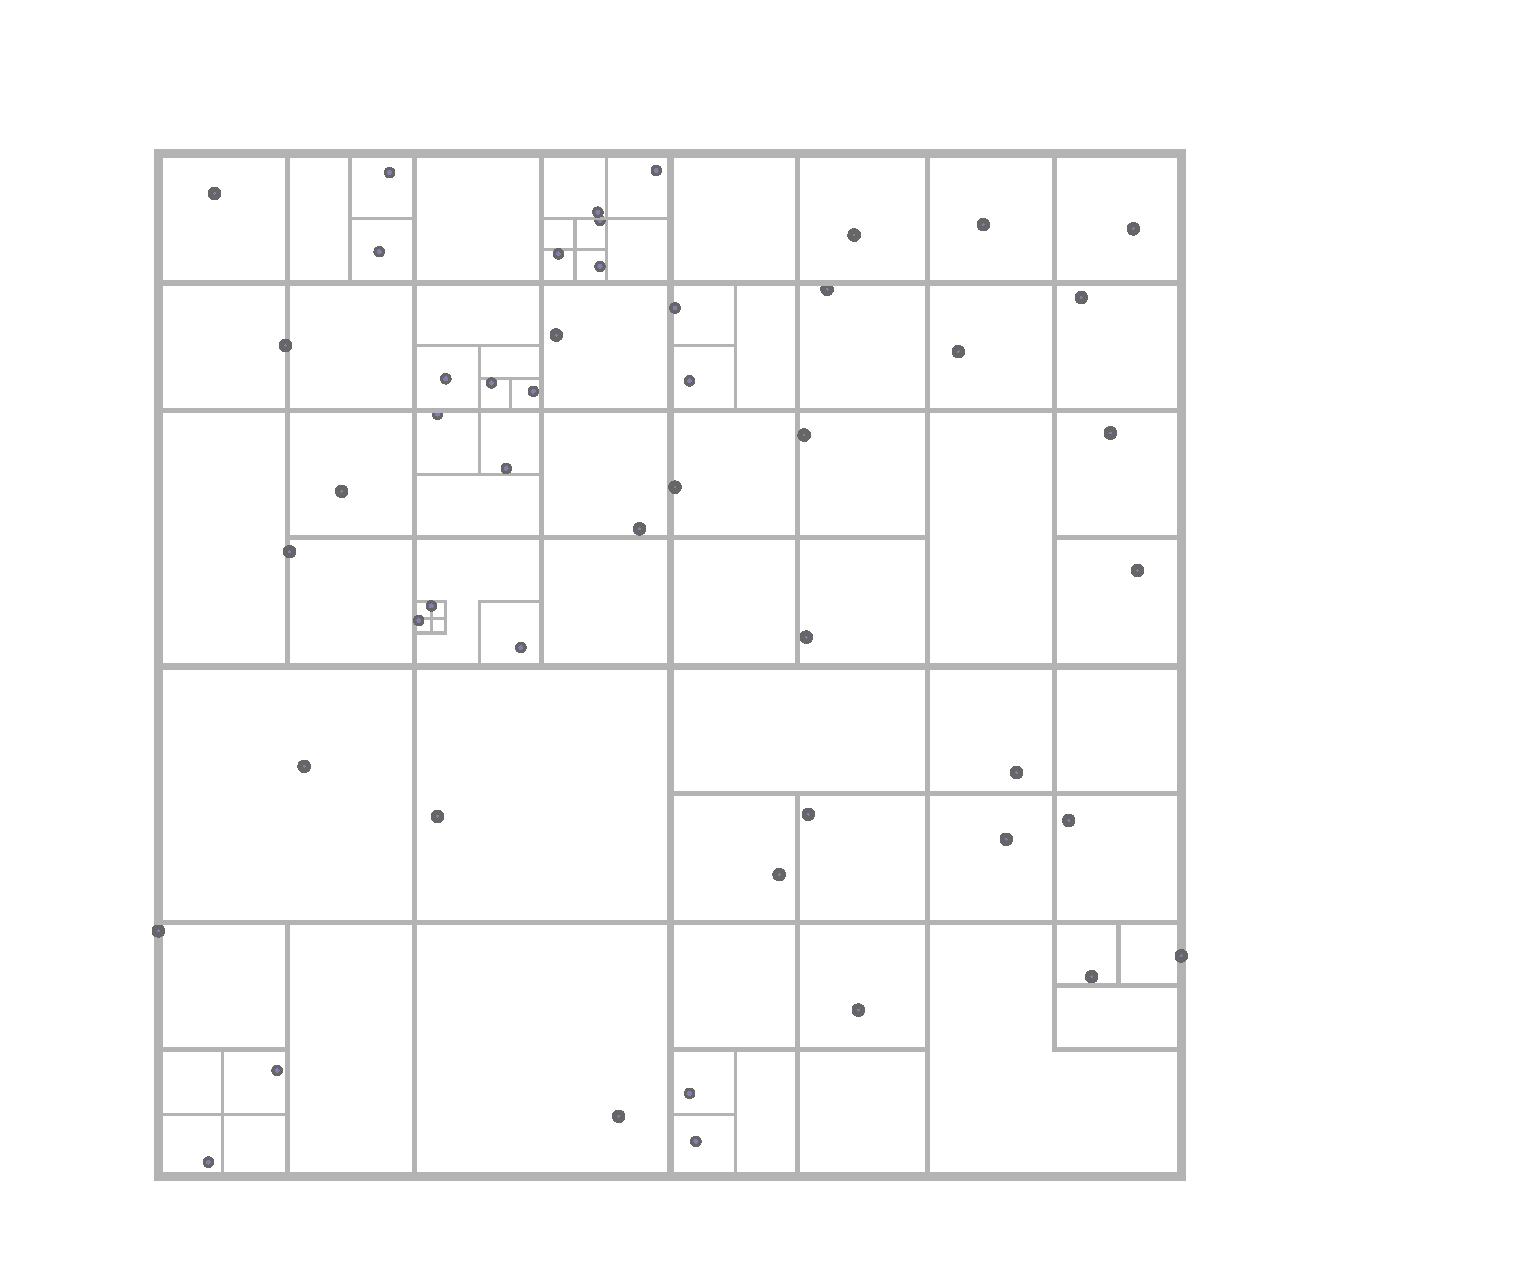
\includegraphics[scale=0.4]{diagrams/compressed_quadtree.eps}
\caption{Compressed Quadtree}
\end{center}
\end{figure}

\begin{thm} \emph{(Height of Compressed Quadtree)}
The height of a compressed quadtree with n points is O(n).
\end{thm}

Compressed quadtrees were first described in \cite{compressedquadtree}, and a
detailed description can be found in \cite{skipquadtree}.

\subsubsection{Z-Order}

TODO: describe z-order, relationship to quadtrees, use to build compressed
quadtree structure.  Outline Chan's algorithm, and the extension to
floating point numbers.

\begin{figure}
\begin{center}
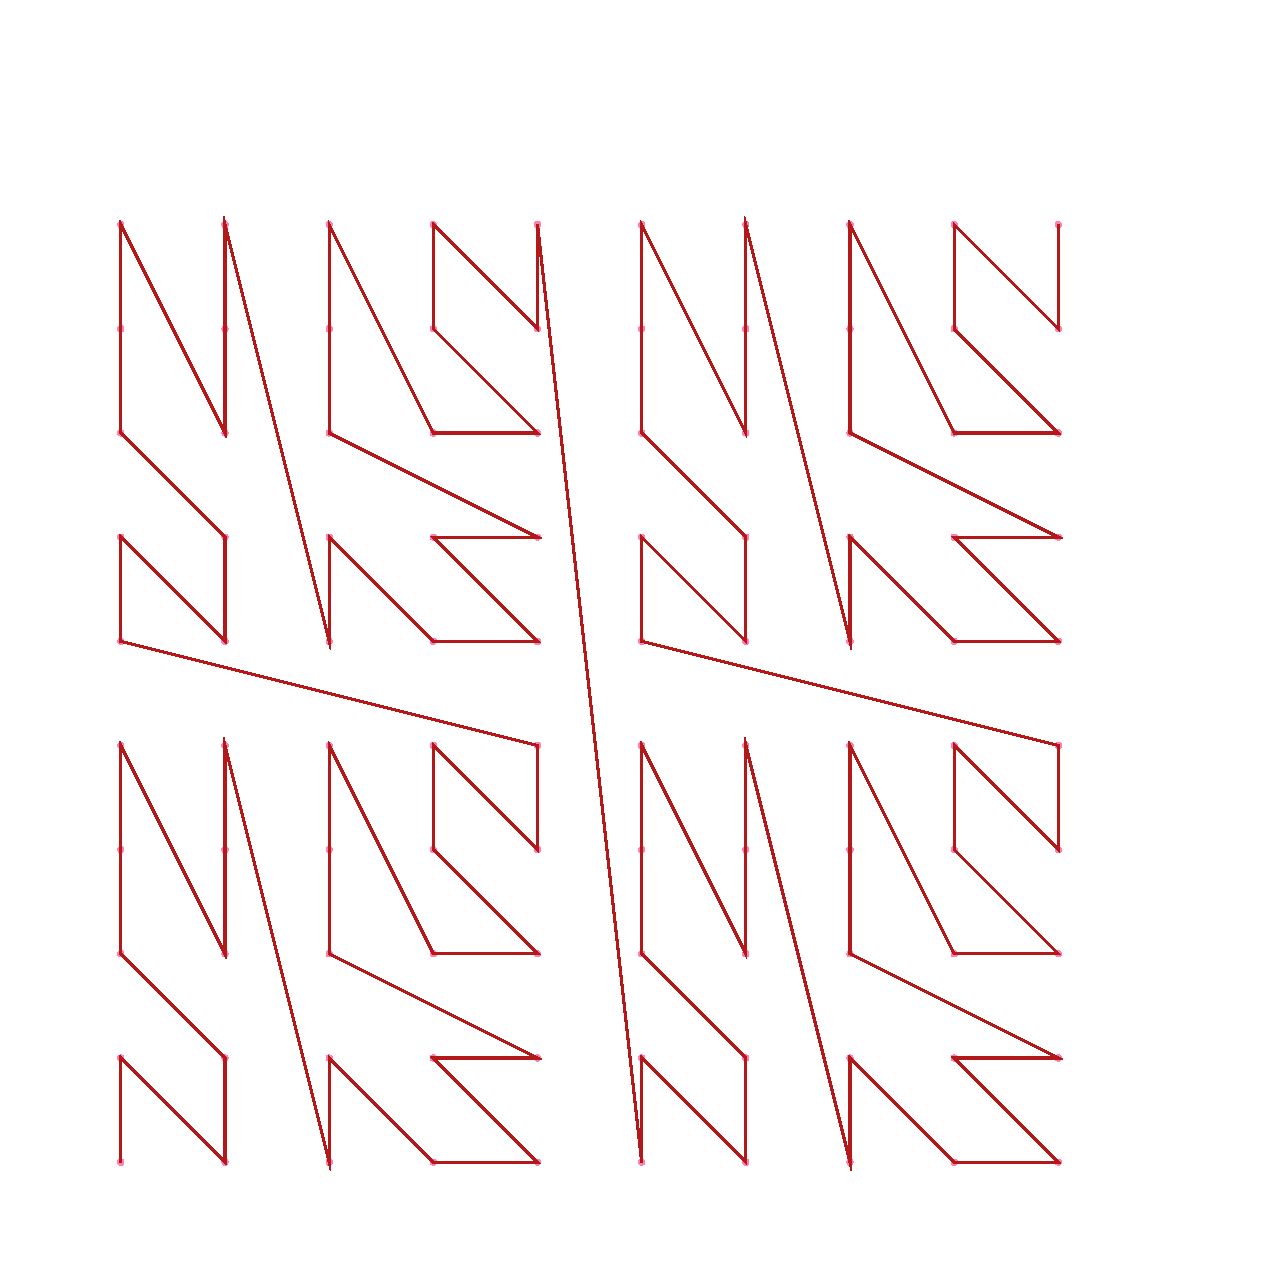
\includegraphics[scale=0.4]{diagrams/zorder.eps}
\caption{Z-Order}
\end{center}
\end{figure}


\subsection{Kd-Trees}

TODO: describe kd-trees, construction procedure, use in nearest-neighbour
search.

\subsection{Partition Trees}

TODO: describe partition trees, construction procedure, use in simplicial
range queries.

\subsection{Odds-on Trees}

TODO: Description of partition tree based Odds-on tree.


\section{Biased Search}

TODO: should this be included here?

\subsection{Biased Search Trees}

Biased search trees are a natural generalization of balancing a binary search
tree where rather than assuming each result is equally likely, a probability
distribution is given for the results, allowing the tree to be balanced such
that at each node it is equally likely that the left or right child will be
followed.  The overall expected running time can then be stated in terms of the
entropy of the probability distribution of the queries.

Early work on biased search trees is described in Knuth \cite{knuth} where
the static case (i.e. no deletions and insertions) is considered.  An \(O(n^2)\)
dynamic programming algorithm is presented which constructs an optimum static
search tree for a set of weights.

Biased search trees allowing insertions and deletions based upon 2 - 4 and
red-black trees were described by Bent, Sleator and Tarjan \cite{bst}.  The
data structures are complex and do not appear to have been implemented.
Feigenbaum and Tarjan describe somewhat simpler data structures \cite{bst2}. A
much simpler implementation of biased search based upon randomized search trees
was developed by Aragon and Seidel \cite{treap}, and a biased version of skip
lists \cite{skiplist} was presented in \cite{bsl2}.

An alternative approach to biased search is to use data structures which
modify themselves in response to queries.  In this case, rather than specifying
the probabilities in advance, the data structure will change itself to match
the query distribution.  Splaytrees \cite{splaytree}, which were invented by
Sleator and Tarjan, are a self-modifying binary search tree which have
received considerable attention, both theoretical and experimental due to the
dynamic optimality conjecture, which states that splaytrees are within a
constant factor of optimal for any sequence of queries, without needing to
know the queries in advance.

Most experimental work with biased search has focused on comparing splaytrees
with traditional approaches like 2 - 4 trees and red-black trees.

TODO: give some references on previous experimental work with biased search.

\subsection{Distribution Sensitive Data Structures}

A distribution sensitive data structure has a running time which is a multiple 
of the entropy of the query distribution.  This is similar to biased search
trees, where the running time is given in terms of the entropy of the query
results, but provides a better framework for examining geometric search
problems.

TODO: Explain why better for geometric search.

TODO: Refer to at least Biased Range Trees paper, some results in distribution
sensitive point location.

\subsection{Instance Optimality}

An instance optimal data structure \cite{chan} has a running time which is
within a constant factor of any data structure for any instance of the problem.

TODO: Explain why this gives equivalent results to distribution sensitive data
structures.

\section{Nearest Neighbour Search}

TODO: Knuth on post-office query, Bentley's quadtrees and kd-trees.  Fast
vector quantization paper, ANN.  Metric trees, Locality sensitive hashing


\chapter{Implementation}

This chapter describes how the odds-on tree was implemented, design decisions
that were made and the performance tuning that was done.

The original description of odds-on trees made use of partition trees.  Although
theoretically optimal, partition trees are not practical to implement, and
implementations were made using both kd-trees and quadtrees.  This chapter
begins with a description of partition tree based odds-on trees, as the
construction and query algorithms are broadly similar to the partition tree
versions.

\section{Kd-tree Implementation}

\section{Kd-tree Based Odds-on Tree}

TODO: Brief overview of kd-tree data structure and how it was implemented.  This
is also the implementation of the back up oracle for both implementations and the
baseline for experimentation. 

\subsection{Construction algorithm}

\subsection{Query algorithm}

\section{Quadtree Based Odds-on Tree}

\subsection{Z-Order and Quadtrees}


\subsection{Construction algorithm}

TODO: Outline how quadtree is built once points are sorted into z-order.

\subsection{Query algorithm}


\section{Performance Tuning}

TODO: Do some profiling to see if there are any spots which can be optimized. 
TODO: Do experimentation to determine appropriate sample size.
TODO: Do experimentation to determine whether or not it is best to sort by NN
      then by z-order or not.

\chapter{Experimental Results}


\section{Experiment Design}

The experimental hypothesis is that the odds-on tree provides better k-nn
performance than a kd-tree implementation in cases where the entropy of the
query set is sufficiently low.

This hypothesis was tested using both synthetic data drawn from probability
distributions, and with data derived from applications of nearest neighbour
search. 

\subsection{Synthetic Data}

\subsubsection{Dimension}

TODO:
- will definitely experiment in 2, 3, 4 dimensions.
- both kd-trees and quadtrees perform poorly in higher dimensions.  The "curse
of dimensionality" says the number of sample points required to build the cache
will grow quickly as dimension increases, but kd-tree performance also quickly
gets worse.
- will try 8, 16 dimensions in a limited number of cases to see if it is worth
while doing full studies.
- above 16 - 20 dimensions, the literature says kd-trees are not effective.
- for exact searches, even 8 dimensions is problematic, not much better than
brute force. 

\subsubsection{Point Set}

The point set

- distribution of points: uniform or mixture of gaussians
- number of points: 10000, 100000, 1000000 

To reduce variance, the point set which was queried to determine the nearest
neighbour was maintained between trials.  Two distributions were used for the

\subsubsection{Sample Set}

The sample set is the set of searches used to build the Odds-on tree.

\subsubsection{Search Set}

The search set is the set of searches used to  test the odds-on tree and
kd-tree implementations.  In all cases, the search set is drawn from the same
distribution used to generate the sample set, and the number of searches was
fixed at 1000000. 

TODO: briefly describe distributions used to generate points: uniform, gaussian,
mixture of gaussians.

\subsection{Application Data}

\subsubsection{Foursquare Dataset}

TODO: describe foursquare dataset, how it is biased, size of dataset, queries
run, etc.

\subsubsection{Photon Mapping Dataset}

Photon mapping is technique used in ray tracing in computer graphics
where lighting is estimated by first creating a photon map by tracing light as
it is emitted from light sources and bounces through the scene, storing the
location each time it hits a surface.  Rays are then traced from the view
location, and each time they hit a surface, the photon map is queried to get an
estimate of the light present at the hit location.  This is a nearest neighbour
search, and it is biased since the queries will only occur on surfaces visible
to the view point, but the photon map will have points for all surfaces visible
to a light source \cite{physicallybased}.

TODO: size of dataset, how to generate a sample dataset, etc.


\section{Measuring Performance}

\subsection{Benchmark Platform}

An Intel Core I5 laptop was used as the benchmark platform.

TODO: Possibly also run experiments on an ARM processor?

\subsection{Performance Metrics}

The primary performance metric is running time.  For each experiment
configuration, 1000000 queries were performed and the elapsed system clock
time was recorded.

In addition to running time, data was collected on the cache miss rate for the
odds-on tree, as well as the number of nodes visited in both the cache and the
back up tree.

Since cache utilization can have a major impact on running time, the Valgrind
\cite{valgrind} cachegrind utility was used to simulate the cache performance
of the implementation, and data was collected on L1 and L2 cache miss rates.

\section{Results}

TODO: one section for each experimental configuration.

\chapter{Conclusion}

\section{Summary}

TODO:

\section{Future Work}

TODO:

\begin{thebibliography}{5}

\bibitem{appnn}
    Arya, S., Mount, D. M., Netanyahu, N. S., Silverman, R. Wu, A. Y. (1998) An Optimal Algorithm for Approximate Nearest Neighbor Searching in Fixed Dimensions , Journal of the ACM, Volume 45, Issue 6, 891--923

\bibitem{ann}
    Mount, D. M., Arya, S. (2010) ANN: A Library for Approximate Nearest Neighbor Searching, retrieved from \url{http://www.cs.umd.edu/~mount/ANN} on Sept. 27, 2010


\bibitem{compressedquadtree}
    Clarkson, Kenneth L. (1983) Fast Algorithms for the All Nearest Neighbors Problem,
FOCS '83: Proceedings of the Twenty-fourth Symposium on Foundations of Computer Science,
Tucson, AZ 
 
\bibitem{treap}
Aragon, C. R.,  Seidel, R. (1996) Randomized Search Trees.
In Algorithmica, Vol. 16, Number 4/5, pp. 464 – 497

\bibitem{skipquadtree}
    Eppstein, D., Goodrich, M. T., Sun, J. Z. (2008) The Skip Quadtree: A Simple Dynamic Data Structure for Multidimensional Data, Int. Journal on Computational Geometry and Applications, 18(1/2), 131--160 

\bibitem{bsl}
Bagchi,A. Buchsbaum, A. L., Goodrich, M. T. (2005) Biased Skip Lists.
In Algorithmica Vol. 42, pp. 31 – 48
 
\bibitem{splaytree}
Sleator, D. D., Tarjan, R. E. (1985) Self-adjusting binary search trees.
In Journal of the ACM, 32, pp. 652 – 686

\bibitem{knuth}
Knuth, D. E. (1998) The Art of Computer Programming, Second Edition,
Volume 3, Sorting and Searching.  Addison-Wesley, Reading, Massachusetts, USA.

\bibitem{bst}
Bent, S. W., Sleator, D. D., Tarjan, R. E. (1984) Biased Search Trees,
In SIAM Journal on Computing, Volume 14, pp. 545 - 568

\bibitem{bst2}
Feigenbaum, J., Tarjan, R. E. (1983) Two New Kinds of Biased Search Tree,
In Bell Systems Technical Journal, Vol. 62, No. 10, pp. 3139 - 3158

\bibitem{skiplist}
Pugh, W. (1990) Skip Lists: A Probabilistic Alternative to Balanced Trees.
In Communications of the ACM, 33(6), pp. 668 – 676

\bibitem{bsl2}
Ergun, F., Sahinalp, S. C., Sharp, J., Sinha, R. K. (2001) Biased Skip Lists
for Highly Skewed Access Patterns, Proceedings of ALENEX 2001, Lecture Notes in
Computer Science, Volume 2153, 216-229

\bibitem{satp}
Williams, H. E., Zobel, J., Heinz, S. (2001) Self-Adjusting Trees in Practice
for Large Text Collections, In Software - Practice and Experience,
Volume 31, pp. 925 - 939

\bibitem{valgrind}
Nethercote, N., Seward, J. (2007) Valgrind: A Framework for Heavyweight Dynamic
Binary Instrumentation.  Proceedings of ACM SIGPLAN 2007 Conference on
Programming Language Design and Implementation (PLDI 2007),
San Diego, California, USA

\end{thebibliography}

\end{document}
